\chapter{Implementation Overview}
In this chapter you should provide a general overview of the project, explaining what you have implemented staying at a high-level of abstraction, without going too much into the details. Leave details for the implementation chapter. This chapter can be organized in sections, such as goal of the project, issues to be solved, solution overview, etc.\\It is very important to add images, schemes, graphs to explain the original problem and your solution. Pictures are extremely useful to understand complex ideas that might need an entire page to be explained.\\Use multiple sections to explain the starting point of your project, the last section is going to be the high-level view of your solution...so take the reader in a short `journey` to showcase your work.

\section{Introduction}
The goal of this project was to design a CMOS-based PUF on a CMOS camera-based device.
The initial phase of the project involved an extensive literature review, to explore the state of the art for CMOS-based PUFs.
After gathering documentation about various implementations, the goal was to identify a reproducible PUF design and then to implement it, using a device of our choice.

\section{Research Process}
The goal of this phase was to identify a well-documented and reproducible PUF design that could serve as a basis for our implementation.
Some material was already available through the project proposal. A comprehensive search through the internet was conducted and led to some other papers
related to PUF technologies and various PUF designs.

The usage of smartphone camera as a PUF basis is a relatively recent field, but a lot of PUF designs have been proposed. From exploiting the randomness of oxide breakdown in CMOS
sensors, to pixel variation noise. Even SRAM memory modules attached to some camera models were exploited to generate PUFs.

A particular implementation emerged as a candidate for the project. It contained a complete description of the design implementation from a mathematical point of view.
The setup used for the experiment validation was well described, together with the theory principles that were at the basis of the design.
The implementation is called CamPUF and the research paper is referenced in [?]


\section{Methodology}
Here are underlined some design choices that were made in order to adapt the implementation to suit the objectives of this project.
The source code is written in \textbf{Python}. This language seemed the optimal choice for the project. It is a general purpose programming language, one of the must popular ones
and for this reason it is rich of extensions, libraries and modules with comprehensive tools to deal with all kinds of paradigms and science fields.
Libraries such as OpenCV, scipy and numpy provided us with the tools to do signal data processing.

A particular challenge was given by the image dataset choice. The program works with RAW images to extract the pixels values. A small dataset of dark images was obtained using a medium-end digital camera (Canon EOS 750D).
A lot of problems were encountered testing this dataset, the hamming distance values with these images were very high, which means that authentication using the same dataset was unsuccessful.
Another small dataset was tested, with raw images provided by an Iphone and the same problem was encountered. 

An explanation for this behavior could be that the images were not completely dark, which means that the DSNU extraction phase captures other type of noise other than DSNU,
leading to a wrong fingerprint or sensors in modern phones could have DSNU removing capabilities, which leads to the same result: a lot of random noise on data extraction.
The choice fell on a dataset provided by the authors of the CamPUF design that used two Android phones from the last decade, plus an application developed by them which uses the Camera2 API.
The DSNU in this dataset was maximized, setting the ISO to the maximum and shutter speed set to the minimum. More information is disclosed in the \underline{\hyperref[chap:results]{Result}} chapter.

\section{Solution Architecture}
\subsection{DSNU Fingerprint Extraction}
The first part of the implementation consists in a Signal Data Processing part, specifically the extraction of the DSNU fingerprint from a couple of frames of a dark image. 
An average of the frames is done to remove temporal noise components and a \textbf{denoising filter} is applied to eliminate noise residual.
A \textbf{DCT Filter} is also used for removing low-frequency components, so that the key generation is based only on high-frequency components, which are discarded in the JPEG compression algorithm.
This simple data processing operations are performed using the external libraries previously mentioned.

\subsection{Enrollment phase}
At this point, the device has generated its DSNU fingerprint and wants to registrate it to the \textit{authenticator} server.
The goal of this phase is to registrate the location of the brightest and darkest pixels of the high frequency component. The indeces of all these locations are stored
and then sent to the authenticator.
\begin{figure}[h!]    
    \centering
    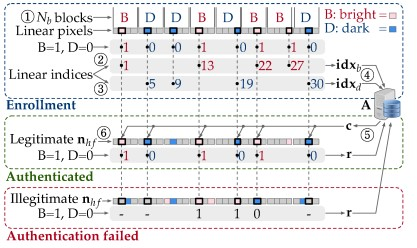
\includegraphics[width=0.5\textwidth]{images/device_auth_flow.jpg}
    \caption{Device authentication flow}
    \label{fig:authflow}
\end{figure}
\subsection{Authentication phase}
This phase is based on comparing the relative brightness of the registered pixels with the response sent from the device. The \textit{Hamming distance} is used as a
metric for measuring the similarity between the two compared keys. A threshold is selected a priori to discriminate between legitimate and illegitimate response.
\\
Figure \ref{fig:authflow} shows the authentication flow of CamPUF.







